\documentclass[paper=a4,fontsize=11pt,DIV=8,BCOR=5mm,twoside,pdftex,bibtotocnumbered]{scrreprt}

%\usepackage{mathptmx}
\usepackage{latexsym,amsmath,amssymb,amsfonts,amsbsy,fancyhdr}
%\usepackage{theorem}
%\usepackage{amsthm}
\usepackage{multirow}
\usepackage{amscd}
\usepackage{enumerate}
\usepackage{mathrsfs}
\usepackage{dsfont}
\usepackage[active]{srcltx}
\usepackage[colorlinks=true, pdfstartview=FitV, linkcolor=black, citecolor=black, urlcolor=black]{hyperref}
\usepackage[dvips]{graphicx}
\usepackage{epsf}
\usepackage{nicefrac}
\usepackage{marvosym}
%\usepackage{subfigure}
\usepackage{caption}
\usepackage{subcaption}
\usepackage{pdfpages}
%\usepackage{fouridx}
%\usepackage{showkeys}
%\usepackage{umlaut}
\usepackage{longtable}
%\usepackage{refcheck}
\usepackage{multirow}
%\usepackage{ulem}
%\usepackage[ngerman]{babel}
%\usepackage{natbib}
%\usepackage{cleveref}
%\crefformat{footnote}{#2\footnotemark[#1]#3}
%\usepackage{biblatex}
%\addbibresource{literature_fraud_detection.bib}
\usepackage{tipx}
\usepackage{setspace}
\usepackage[ruled]{algorithm2e}
\usepackage{amsthm}
\onehalfspacing

%\let\origdoublepage\cleardoublepage
%\newcommand{\clearemptydoublepage}{%
%  \clearpage
%  {\pagestyle{empty}\origdoublepage}%
%}

%\cleardoublepage
%\clearemptydoublepage

\usepackage{graphicx}
\usepackage[justification=centering]{caption}

\usepackage{pgfplots}
\pgfplotsset{width=10cm,compat=1.8}

\newcommand{\R}{{\mathbb R}}
\newcommand{\rp}{\R^+}
\newcommand{\rpn}{\R^+_0}
\newcommand{\C}{{\mathbb C}}
\newcommand{\N}{{\mathbb N}}
\newcommand{\Z}{{\mathbb Z}}
\newcommand{\Q}{{\mathbb Q}}

\newcommand{\rarrow}{\Longrightarrow}
%\newcommand{\larrow}{\Longleftarrow}
%\newcommand{\lrarrow}{\Longleftrightarrow}
%\newcommand{\lir}{``$\rarrow:$''\,}
%\newcommand{\ril}{``$\larrow:$''\,}

\renewcommand{\P}{{\mathbb P}}
\newcommand{\E}{{\mathbb E}}
\newcommand{\var}{\text{Var}}
\newcommand{\iid}{\text{i.i.d.} }
\newcommand{\dct}{\text{DCT}}
\newcommand{\mct}{\text{MCT}}
\renewcommand{\d}{\text{ d}}
\newcommand{\dd}{{\rm d}}
\newcommand{\rcll}{\text{RCLL}}
\newcommand{\diam}{\text{diam}}
\newcommand{\degree}{\text{deg}}
\usepackage{amsmath}
\DeclareMathOperator*{\argmax}{arg\,max}

\newcommand{\comment}[1]{\marginpar{\textcolor{red}{#1}}}
%\newcommand{\clearemptydoublepage}{\newpage{\pagestyle{empty}\cleardoublepage}}
%\newcommand{\emptydoublepage}{\newpage{\pagestyle{myheadings}\pagestyle{myheadings}\markboth{}{}\cleardoublepage}}

%\newcommand{\argmin}{{\rm argmin}}

\renewcommand{\matrix}[1]{\mathbf{#1}}
\renewcommand{\vec}[1]{\mathbf{#1}}
\newcommand{\refEqu}[1]{(\ref{#1})}

\newcommand{\package}{{\sl trustpay}}

%\newtheorem{algorithm}{Algorithm}
\theoremstyle{plain}
\newtheorem{thm}{Theorem}
\newtheorem{proposition}{Proposition}
\newtheorem{corollary}[proposition]{Corollary}
\newtheorem{lemma}[proposition]{Lemma}
%\theorembodyfont{\rm}
\newtheorem{definition}[proposition]{Definition}
\newtheorem{example}[proposition]{Example}
\newenvironment{ex}{\begin{example}}{\hfill$\lozenge$\end{example}}
\newtheorem{rem}[proposition]{Remark}
\newenvironment{remark}{\begin{rem}}{\hfill$\lozenge$\end{rem}}
\newtheorem*{myproof}{Proof}
\newcommand{\theproof}{}
\newenvironment{pf}{\begin{myproof}}{\hfill$\square$\end{myproof}}
\newtheorem{hypothesis}{Hypothesis}

%\pagestyle{headings} \rfoot{edsg}
\pagestyle{plain}
\oddsidemargin=-0.1ex
\evensidemargin=-0.1ex
\textheight=23cm
\textwidth=16.5cm
\topmargin=-1.5cm
\oddsidemargin=0cm
%\parindent0cm
\parskip1ex

\RequirePackage{makeshape} 
\RequirePackage{tikz}
\usetikzlibrary{shapes}
\usepackage{flowchart}
\usetikzlibrary{arrows}
\usetikzlibrary{positioning}

%\usepackage[
%backend=biber,
%style=alphabetic,
%sorting=ynt
%]{biblatex}
%\addbibresource{literature_payment_assignment.bib}
%\usepackage[nottoc]{tocbibind}

\allowdisplaybreaks

\DeclareMathAlphabet{\mathcal}{OMS}{cmsy}{m}{n}

\usepackage{hyperref}

\begin{document}
\begin{titlepage}
	\begin{center}
		\Huge \textsf{\textbf{Identifiying cancer subtypes using graph-based clustering}}
		\\[1.4cm]
		\Large \textsf{\textbf{Lena Zuspann}}
		\\[1.4cm]
		\today
	\end{center}
\end{titlepage}

\setcounter{page}{1}
\tableofcontents

\chapter{Introduction}\label{ch:intro}
In molecular biology, the goal is to understand the molecular bases of biological activity in and between cells. It has its origins in the 1950s when the double-helix structure of DNA was introduced and soon after, genes located in DNA could be transcribed to RNA. RNA is short for Ribonucleic acid which is a molecule that is responsible for a lot of biological functions, either directly (non-coding RNA) or by enableing the production of according proteins (messenger RNA or m-RNA). The study of RNA, which in literature is also refered to as the transcriptome, is particularly useful for analysing functions of genes, identifying molecular compositions of cells, and understanding the cause and development of diseases. Over the past few decades, researchers have come up with various methods to get an in-depth analysis of RNAs and a more better understanding of gene expression. This has led to the introduction of RNA-sequencing which now gives biologists the opportunity to process and map transcriptome by the use of gene expression levels that can detect the presence and quantitiy of RNA in a biological sample. A quantified RNA-sequencing result is a snapshot at a given time and can be used to detect anomalies in the underlying biological sample. 

Nowadays in cancer research, RNA-sequences can be used to identify different forms of cancer. However, to make the treatment as effective as possible it is important to identify tumor subtypes and to develop more personalized theorapies. Biologically, this is a challenging task especially in view of the huge amounts of data that can be obtained by all kinds of sequencing technologies. Furthermore, the goal is to identify connections and similarities in the data that were not obtained by theoretical analyses before. This is the reason why algorithmic approaches, in particular clustering algorithms, can be helpful. 

In this particular project, we focus on the HCS (highly connected subgraphs) clustering algorithm, which was introduced in \cite{Hartuv2000}, that makes use of graph connectivity for cluster analysis. It stores the data set in a similarity graph where the data points are represented as vertices and the edges between them represent their similarity. The algorithm works iteratively by using the minimum cut of the graph to partition it and to ultimately identify HCS as clusters. 

More specifically in Chapter~\ref{ch:theory}, we first theoretically describe this clustering algorithm, determine its running time and analyse its properties, in particular we show that the groups of the clustering result have a high homogenity within the group and a high seperation with respect to every other group which are the desired properties of a clustering procedure. Then, we introduce an algorithm to determine the minimum cut of a given graph in a weighted, undirected graph and determine its running time. The last part of the theoretical chapter consists of two approaches to construct a similarity graph from a given data set. We explain how they work and provide their running times.

In Chapter~\ref{ch:implementation}, we document the implementation of the previously described algorithms in a Python project. First, we give an overview of the gene expression cancer RNA-Seq data set\footnote{The data set can be downloaded at \url{https://www.synapse.org/Synapse:syn4301332}.} we are using for this purpose. Then, we describe the construction of the corresponding similarity graph and discuss the implemenation of the HCS clustering algorithm. Additionally, we provide a praxis-oriented solution for a common problem of the clustering result for the data set under consideration that is also implemented in the project.

Finally in Chapter~\ref{ch:discussion}, we discuss the results and improvements of the different approaches for specific examples of the clustering results.

\chapter{Theoretical description of the algorithm}\label{ch:theory}

\section{Introduction of general terms}\label{sec:intro_def}
In this section, we give the definitions of some important terms in graph theory that are necessary to describe the algorithm we use in this project.

\begin{definition}[Undirected graph]
	An \emph{undirected graph} is a pair $G := (V, E)$ which consists of the set of vertices $V$ and the set of edges $E$. Edges are defined as a set of paired vertices.
\end{definition}

\begin{definition}[Path]
	A \emph{path} $p$ in a graph $G$ is a sequence of edges which joins sequence of pairwise distinct vertices. We denote a path from $u\in V$ to $v\in V$ with $p := (u, u_1, u_2, \dots, v)$, where $u_i \neq u_j$ for all $i\neq j$.
\end{definition}

\begin{definition}[Minimum degree of a graph]
	Given a graph $G=(V,E)$, we define the \emph{degree} $\degree(v)$ of a vertex $v\in V$ as the number of edges incident with it. The \emph{minimum degree} among all vertices in a graph is denoted be $\delta(G)$.
\end{definition}

\begin{definition}[Connected graph]
	Let $G$ be an undirected graph. We call two vertices $u,v \in V$ connected if there exists a path from $u$ to $v$ in $G$. Otherwise, we call them disconnected. \\
	If every pair of vertices in $G$ satisfies this property, we call the graph $G$ \emph{connected}. Otherwise, we call it disconnected.
\end{definition}

\begin{definition}[Connectivity of a graph]
	The \emph{connectivity} of graph $G$, denoted by $k(G)$, is the minimum number of edges which when removed lead to a disconneted graph. If $k(G) = l$, the graph $G$ is called \emph{$l$-connected}. \\
	Let $n = |V|$ be the number of vertices of $G$. If $k(G) > \frac{n}{2}$, we call the graph $G$ \emph{highly connected}.
\end{definition}

\begin{definition}[(Minimum) cut]
	Given a graph $G = (V, E)$, a \emph{cut} $C := (S, T)$ is a partition of $V$ into to subsets $S$ and $T$. The \emph{cut set} $\mathcal{C}$ corresponding to $C$ is the set of all edges in $E$ that have one endpoint in $S$ and the other in $T$: $\{(u,v) \in E : u \in S, v \in T\}$. We define the \emph{size} of a cut $s(C) := |\mathcal{C}|$ as the cardinality of the cut set. A \emph{mininum cut} of a graph is a cut of minimal size.
\end{definition}

\begin{definition}[Clique]
	Given a graph $G=(V,E)$, a subset of vertices $C \subset V$ is called \emph{clique} if for all pairwise distinct vertices $u, v \in C$ there exists an edge $(u,v) \in E$.
\end{definition}

\section{The HCS algorithm}\label{sec:hcs}
The highly connected subgraph (HCS) algorithm is a recursive procedure that takes as an input a graph $G=(V,E)$ and returns a collection of highly connected subgraphs. It uses minimum cuts to divide the original graphs into subgraphs and then checks if those are highly connected. Single vertices are not considered as a valid subgraph and thus collected in a singletons set. 

Below, we show the pseudocode of the procedure as shown in \cite{Hartuv2000}, assuming that the algorithm MINIMUM-CUT($G$) returns $H$, $\bar{H}$ and $C$, where $C$ is the minimum cut separating $G$ into the subgraphs $H$ and $\bar{H}$.

\begin{algorithm}
	\caption{HCS($G$)}\label{alg:hcs}
		$(H, \bar{H}, C) \gets \text{MINIMUM-CUT}(G)$\\
		\eIf{$G$ is highly connected}
			{\Return $G$}
			{ 
			HCS($H$)\\
			HCS($\bar{H}$)}
\end{algorithm}

Let $N$ be the number of clusters found. Then, the running time is bounded by $2N \cdot f(n,m)$, where $f(n,m)$ denotes the running time of the MINIMUM-CUT algorithm for a given graph $G$ with $n$ vertices and $m$ edges. Note that in most applications $N \ll n$.

\section{Properties of the HCS algorithm}\label{sec:properties_HCS}
In clustering, the aim is to assign data points into groups that have a high homogenity within the group and a high seperation with respect to every other group. In this section, we provide some results showing that the HCS algorithm has these properties.

\begin{definition}[Diameter of a graph]
	Given a graph $G = (V,E)$, we define the \emph{distance} $d(u,v)$ between any two vertices $u, v \in V$ as the number of edges (length) of the shortest path joining them. If such a path does not exist, we define $d(u,v) := \infty$. Now, assume that $G$ is a connected graph. Then, we define the \emph{diameter} of $G$, denoted as $\diam(G) :=\underset{u,v \in V}{\argmax} \,d(u,v)$ between any two vertices in $G$.
\end{definition}

By this definition, we can observe that the diameter of a graph gives us an indiction of how close the data points in a graph are, assuming that we view closeness as how many edges a path between two vertices has. Given data points that we want to cluster, the graph to which we apply the HCS algorithm is a similarity graph. Homogenity of a cluster in this context means that the highly connected subgrahs resulting from the algorithm have small diameter. This propety is the result of the following theorem.

\begin{thm}\label{thm:diameter_highly_connected_subgraph}
	The diameter of every highly connected graph is at most two.
\end{thm}

\begin{pf}
	This proof follows the lines of Theorem~1 in \cite{Hartuv2000}.\\
	Given a graph $G=(V,E)$ with connectivity $k(G)$, this means by definition that we need to remove at least $k(G)$ edges to obtain a disconnected graph. Assume $G$ has minimum degree $\delta(G)$. If we consider a vertex $\in V$ whose degree is equal to the minimum degree of the graph, i.e. $\deg(v) = \delta(G)$, and remove all of its incident edges the result is a disconnected graph. Thus, we know that $k(G) \le \delta(G)$. If $G$ is also highly connected, by definition we get
	\[
	\frac{|V|}{2} < k(G) \le \delta(G).
	\]
	This means that every vertex is adjacent to at least half of the vertices of $G$. Hence, every pair of vertices has a common neighbor and as a result their distance is at most two.
\end{pf}

This is a strong indication of homogenity within a cluster since the only better situation in terms of the diameter would be one which means that every pair of vertices has an edge connecting them. But this would mean that there can't be any false positives in the similarity graph and it would require to solve the clique-problem which is NP-hard.

The following theorem gives another strong implication of homogenity.

\begin{thm}\label{thm:quadratic_cluster_size}
	The number of edges in a highly connected subgraph is quadratic.
\end{thm}

\begin{pf}
	This proof follows the lines of Theorem~4(a) in \cite{Hartuv2000}.\\
	Let $G=(V,E)$ be a highly connected subgraph with $n = |V|$ vertices. Using the inequality $\frac{n}{2} < k(G) \le \delta(G)$ from the proof of Theorem~\ref{thm:diameter_highly_connected_subgraph}, we can give a lower bound on the total number of edges as follows
	\[
	|E| \ge \delta(G) \cdot n \cdot \frac{1}{2} > \frac{n}{2} \cdot n \cdot \frac{1}{2} = \frac{n^4}{2},
	\]
	where the first inequality results from the fact that the number of total edges in $G$ is at least the amout of edges that a graph has where every vertex is of minium degree $\delta(G)$.
\end{pf}

In the following, we will consider a few theorems that indicate that the clustering resulting from the HCs algorithm also has the seperation property. First, we consider the following Lemma that is needed to prove the theorems.

\begin{lemma}\label{lem:min_cut_clique}
	Let $G=(V,E)$ be a graph and $S$ be a minimum cut that splits $G$ into two induced subgraphs $H$ and $\overline{H}$, respectively. Without loss of generality, we assume that $1 < k := |V(\overline H)| < |V(H)|$. Then, $|S| \le k$ with equality only in the case in which $\overline{H}$ is a clique.
\end{lemma}

\begin{pf}
	This proof follows the lines of Lemma~2 in \cite{Hartuv2000}.\\
	We denote by $\degree_H(v)$ the degree of vertex $v\in V(H)$ and by $\degree_S(v)$ the number of edges in $S$ that are incident on $v$. We defined $S$ to be a minimum cut which means that, for every $v \in V(\overline{H})$, we have 
	\[
	\degree_{\overline{H}}(v) + \degree_S(v) \ge |S|.
	\]
	Otherwise, $\tilde{S}:= (V, V\backslash\{v\})$ would be a minimum cut with $|\tilde{S}| < |S|$ which is a contradiction. Summing over all vertices in $V(\overline{H})$, we get 
	\[
	\begin{aligned}
	\sum_{v\in \overline{H}} \degree_{S}(v) + \sum_{v\in \overline{H}} \degree_{\overline{H}}(v) &\ge |S| |V(\overline H)| \\
	\Longleftrightarrow |S| + 2|E(\overline{H})| &\ge |S| |V(\overline H)| \\
	\Longleftrightarrow 2|E(\overline{H})| &\ge |S| (|V(\overline H)| - 1).
	\end{aligned}
	\] 
	Now, if $|V(\overline H)|>1$, we get
	\[
	\begin{aligned}
	|S| &\le \frac{2|E(\overline{H})|}{|V(\overline H)| - 1} \\
	&\le \frac{2\left(\frac{|V(\overline H)| (|V(\overline H)| - 1)}{2}\right)}{|V(\overline H)| - 1} \\
	&= |V(\overline H)| =: k,
	\end{aligned}
	\]
	where in the first step we divided by the right-hand side from above that by assumption is greater than zero. In the second step, we used the fact that in a graph the number of edges is upper bounded by the number of edges in a graph where each pairwise distinct vertices are adjacent, i.e. the number of edges in a clique.
	In the case of $|S| = k$, both inequalities of the above equation must be equalities, i.e. 
	\[
	|E(\overline{H})| = \frac{|V(\overline H)| |V(\overline H)| - 1}{2},
	\]
	which implies that $\overline H$ is a clique.
\end{pf}

\begin{thm}\label{thm:diameter_clique}
	Let $G=(V,E)$ be a graph that has diameter two but is not highly connected. Denote by $H$ and $\overline{H}$ the induced subgraphs obtained by removing a minimum cut $S$ from $G$. Assume that $|V(\overline H)| \le |V(H)|$, where $V(\overline H)$ and $V(H)$ denote the set of vertices of $\overline H$ and $H$, respectively. Then,
	\begin{enumerate}
		\item every vertex in $\overline H$ is incident on $S$.
		\item $\overline H$ is a clique, and
		\item if $|V(\overline H)|>1$ then every vertex in $V(\overline H)$ is incident on a single edge of $S$.
	\end{enumerate}
\end{thm}

\begin{pf}
	This proof follows the lines of Theorem~3 in \cite{Hartuv2000}.\\
	We divide this proof into two different cases.
	
	\textbf{Case 1} $\left(|S| = \frac{|V|}{2}\right)$\textbf{.} If $V(\overline{H}) = 1$, it follows directly that the theorem is true since a graph with only one vertex is a clique and this single vertex in $\overline{H}$ had to be connected before the removal which implies statement (1). Hence, suppose  $V(\overline{H}) > 1$. Lemma~\ref{lem:min_cut_clique} then implies that both $H$ and $\overline{H}$ are cliques with $|V(\overline H)| = |V(H)| =  \frac{|V|}{2}$ vertices. This immediately implies (2). 
	
	To show (1), we now assume that there exists $v\in V(\overline H)$ such that $v$ is not incident on $S$. Then, $\degree(v) < \frac{|V|}{2}$ which would mean that $\tilde{S}:= (V, V\backslash\{v\})$ would be a minimum cut with $|\tilde{S}| < |S|$ and this is a contradiction. 
	
	(3) now follows since by (2) $S$ contains as many edges as there are in each of the induced subgraphes $H$ and $\overline{H}$, respectively, and by (3) every vertex in $V(\overline H)$ is incident to at least one edge in $S$, which implies that every vertex in $V(\overline H)$ can only be incident on a single edge of $S$.
	
	\textbf{Case 2} $\left(|S| < \frac{|V|}{2}\right)$\textbf{.} First, we show that $|V(\overline H)| < |V(H)|$. Suppose that $|V(H)| = |V(\overline H)| = \frac{|V|}{2}$, i.e. by assumption $|S| < |V(H)|$ and $|S| < |V(\overline H)|$. Hence, there exist $u \in V(H)$ and $v\in V(\overline{H})$ such that $u$ is not adjacent to any vertex in $V(\overline{H})$ and $v$ is not adjacent to any vertex in $V(H)$. But this implies that $d(u,v) > 2$ which is a contradiction to the initial assumption $\diam(G) \le 2$.
	
	Since then $V(H)| > \frac{|V|}{2} > |S|$, there exists a vertex $u \in V(H)$ that is not incident on $S$. If there also exists a vertex $v\in V(\overline{H})$ that is not incident on $S$, this would again imply $d(u,v) > 2$, i.e. a contradiction to $\diam(G) \le 2$. This concludes that (1) holds.
	
	By (1), we know that $|V(\overline{H})| \le |S|$. If $|V(\overline{H})| = 1$, (2) follows directly since a graph with only one vertex is a clique. Now, suppose that $|V(\overline{H})| > 1$. Using Lemma~\ref{lem:min_cut_clique}, we get that $|S| \le |V(\overline{H})|$. Putting those two inequalities together, we get that $|S| = |V(\overline{H})|$. The second part of Lemma~\ref{lem:min_cut_clique} then implies (2) and (3) also follows since there are as many edges in $S$ as vertices in $\overline{H}$ which means exactly one each.
\end{pf}

The above theorem gives an indication of the seperation property of the HCS algorithm's result when considering the following situation. Let $G=(V,E)$ be the similarity graph that the algorithm starts with. Now suppose that at some point the algorithm splits the subgraph $\tilde{G}$ with $\diam(\tilde{G})$ into the non-trivial sets $C_1$ and $C_2$ which without loss of generalty we assume to satisfy the property $t = |C_1| \le |C_2|$. Let $S$ be the minimum cut causing this particular split. Using Theorem~\ref{thm:diameter_clique}, we know that each vertex in $C_1$ is incident to $S$ and adjacent to one single vertex in $C_2$. 

Now, we want to consider the likeliness of $\tilde{G}$ being a true cluster or a subset of one given this minimum cut $S$. Since $|C_2| \ge t$, it follows that in the true cluster containing $C_1 \cup C_2$ only $t$ out of all the edges between $C_1$ and $C_2$ are present due to the properties of $S$ discussed above. But again by Theorem~\ref{thm:diameter_clique}, $C_1$ is a clique since it is the smaller set resulting from the removal of the minimum cut and thus all of the $t \choose 2$ edges are present. This means that unless $t$ is very small, this is a situation very unlikely to be caused by some random noise within a cluster. Hence, any non-trivial set split by the HCS algorithm is unlikely to have diameter two but instead at least diameter three.

In the following, we view another theorem that indicates the seperation property of the solution given by the HCS algorithm.

\begin{thm}
	The number of edges removed by each iteration of the HCS algorithm is at most linear.
\end{thm}

\begin{pf}
	Let $G=(V,E)$ be a graph with $n=|V|$ vertices. In each iteration, the HCS algorithm splits the graph $G$ into two components. This means that the number of edges between those two components is at most $\frac{n}{2}$.
\end{pf}

Hence, while the number of edges in the final clusters is quadratic in the size of the underlying subclusters according to Theorem~\ref{thm:quadratic_cluster_size}, the above theorem states that the number of edges removed by each iteration of the HCS algorithm is linear. Thus, unless the sizes are very small this indicates seperation between the clusters.

\section{MINCUT algorithm}\label{sec:mincut}
The way in which we introduced a minimum cut in Section~\ref{sec:intro_def} and the setting in which we want to apply the algorithms suggests that we are considering the minimum cut problem for undirected graphs. In this case, we can make use of the Stoer-Wagner minimum cut algorithm which is limited to non-negative edge weights but in Section~\ref{sec:sim_graphs}, we will see that this restriction does not cause any problems in our use case. Before we get to the specific steps of the algorithm, we would like to introduce a few additional terms.

\begin{definition}[$s-t$ cut and $s-t$ min-cut of a graph]
	Let $G=(V,E)$ be an undirected graph and let $s,t \in V$. We call a cut $C=(S,T)$ an \emph{$s-t$ cut} if exactly one of $s$ or $t$ is in $S$. Let $\tilde{C}$ be the minimum cut of $G$. If it is also an $s-t$ cut we call $\tilde{C}$ the \emph{$s-t$ min-cut} of $G$.
\end{definition}

The algorithm is built upon the following theorem.

\begin{thm}
	Let $G=(V,E)$ be a weighted, undirected graph\footnote{This theorem also applies to unweighted, undirected graphs by giving all existing vertices weight one.} and let $s,t \in V$. Define $G\backslash\{s,t\}$ as the graph obtained by merging $s$ and $t$. More specifically, this means that in $G\backslash\{s,t\}$, $s$ and $t$ are merged into a new vertex $st$. All edges between $s$ and $t$ in $E$ are deleted and if there are any other vertices connecting either $s$ or $t$ or both of them to another vertex $v\in V$, these will be replaces by an edge $(st, v)$ with weight $w(s,v) +  w(t,v)$. Note that one of those weights can be zero.
	
	Then, a minimum cut $G$ can be obtained by taking the smaller of a $s-t$ min-cut of $G$ and a min-cut of $G\backslash\{s,t\}$.
\end{thm}

\begin{pf}
	This proof follows the lines of Theorem~2.1 in \cite{Stoer1997}.\\
	Given $G$ and two vertices $,t\in V$, one of the following two cases applies: either there is a minimum cut of $G$ that separates $s$ and $t$ or if not, there $s$ and $t$ are on the same side of any minimum cut of $G$ which then also has to be a minimum cut of $G\backslash\{s,t\}$.
\end{pf}

This theorem implies that we can use finding an arbitrary $s-t$ min-cut to construct a recursive procedure to find a min-cut of the graph. The Stoer-Wagner algorithm is split into two parts. The first one is called MINIMUM-CUT-PHASE\footnote{This algorithm is also known as maximum adjacency search or maximum cardinality search.}.

\begin{algorithm}
	\caption{MINIMUM-CUT-PHASE}\label{alg:min_cut_phase}
	\KwIn{$G=(V,E)$ input graph; $w$ weight function; $a\in V$ starting vertex}
	\KwOut{cut-of-the-phase, $\tilde{G}$ shrinked input graph}
	$A \gets \{a\}$\\
	\While {$A \neq V$}
		{add the most tightly connected vertex to $A$, i.e. $A \gets A \cup \{z\}$, where $z \notin A$ such that $w(A, z) = \max \{w(A,y) | y \notin A\}$ and where $w(A,y)$ is the sum of all edges between $A$ and $y$}
	cut-of-the-phase $\gets$ cut of $V$ that separates the vertex added last from the rest of the graph\\
	$\tilde{G} \gets G\backslash\{s,t\}$, where $s,t \in V$ are the two vertices added last to $A$
\end{algorithm}

Algorithm~\ref{alg:min_cut_phase} returns a $s-t$ min-cut in the input graph $G$, where $s, t \in V$ are the two vertices added last to the set $A$ which can be seen in more detail in \cite[Lemma~3.1]{Stoer1997}. The above algorithm will be applied multiple times to a shrinking input graph $G$ in the second part of the procedure called MINIMUM-CUT given below.

\begin{algorithm}
	\caption{MINIMUM-CUT}\label{alg:min_cut}
	\KwIn{$G=(V,E)$ input graph; $w$ weight function; $a\in V$ starting vertex}
	\KwOut{minimum-cut}
	\While {$|V| > 1$}
	{cut-of-the-phase, $G \gets$ MINIMUM-CUT-PHASE($G$, $w$, $a$)\\
	\If{cut-of-the-phase is ligther than the current-minimum-cut}
	{store the cut-of-the-phase as the current-minimum-cut}}
	minimum-cut $\gets$ current-minimum-cut
\end{algorithm}

Note that the starting vertex stays the same throughout the whole algorithm. For a randomized approach, $a$ could also be chosen randomly in each phase instead. The running time of Algorithm~\ref{alg:min_cut} is due to the while loop equal to $|V|-1$ runs of Algorithm~\ref{alg:min_cut_phase}. For an efficient implementation of the latter the way of selecting the next vertices to add to the set $A$ is important. All the vertices not yet added to $A$ are stored in a priority queue based on keys, where the key for a vertex $v\in V\backslash A$ is $w(A,v)$, i.e. the weights of the edges connecting it to the current $A$. Adding another vertex to $A$ means that we need to find the vertex with the maximum key in the queue, i.e. $u := \underset{v\in V\backslash A}{\argmax} \, w(A,v)$, extract it (in total $|V|$ times) and increase the keys of all other vertices $w \in V\backslash A$ connected to $u$ by $w(w,u)$ (in total $|E|$ times). Using Fibonacci heaps as in \cite{Fredman1987}, extracting the maximum can be done in $\mathcal{O}(\log |V|)$ and increasing the key in $\mathcal{O}(1)$ amortized time. This means that one call of Algorithm~\ref{alg:min_cut_phase} has a running time of $\mathcal{O}(|E| + |V| \log |V|)$ and thus, we get a total running time of $\mathcal{O}( |V| |E| + |V| ^2\log |V|)$.

\section{Similarity graphs}\label{sec:sim_graphs}
The HCS algorithm takes as an input a graph but in our use case we consider a tabular data set. To transform this data set in a way that the clusters obtained from the algorithm give useful information about the original data, we use similarity graphs. In this section, we first introduce the concept of similarity graphs and then show two approaches to construct them from a given tabular data set.

\begin{definition}[Distance metric]\label{def:dist_metric}
	Let $M$ be a set and let $d: M \times M \rightarrow \R$ be a function satisfying the following properties:
	\begin{enumerate}[(1)]
		\item Well-defined: For all $x\in M$, we have $d(x,x)=0$.
		\item Positivity: For all $x, y\in M$ with $x\neq y$, we have $d(x,y)>0$.
		\item Symmetry: For all $x,y\in M$, we have $d(x,y) = d(y,x)$.
		\item Triangle inequality: For all $x,y,z\in M$, we have $d(x,z) \le d(x,y) + d(y,z)$.
	\end{enumerate}
	Then, we call $d$ a \emph{metric} on $M$ and the ordered pair $(M,d)$ \emph{metric space}.
\end{definition}

When one wants to quantify the similarity of two data points intuitively this would mean some sort of inverse of the distance, i.e. the smaller the distance the higher the similarity. Mathematically, there does not exist a proper definition of similarty but we keep the intuition about similarity in mind and consider the following:

\begin{definition}[Gaussian kernel]\label{def:Gaussian_kernel}
	Given a metric space $(M,d)$ where $M=\R^n$, $n\in\N$, and $d(\cdot, \cdot):= \lVert \cdot - \cdot \lVert^2$ is the Euclidean distance, we define the \emph{Gaussian kernel} for $x,y\in M$ as follows:
	\[
		k(x,y) := \exp\left\{-\frac{\lVert x-y \rVert^2}{2\sigma^2}\right\} \in (0,1]
	\]
	for some $\sigma^2 \in \R^+$.
\end{definition} 

Notice that the Gaussian kernel is some non-linear function of the Euclidean distance which decreases with distance. Now, since our goal is to connect data points that are similar to each other, using the Gaussian kernel for some appropriate variance parameter $\sigma^2\in\R^+$ is reasonable. Given data points from some tabular data set, we can construct a graph using Algorithm~\ref{alg:eps_sim_graph}.

\begin{algorithm}
	\caption{$\epsilon$-neighborhood similarity graph}\label{alg:eps_sim_graph}
	\KwIn{$\{x_i\}_{i \in \{1,\dots, n\}}$, $n\in\N$ data points; $\epsilon\in[0,1)$ and $\sigma^2\in\R^+$ parameters}
	\KwOut{$G=(V,E)$ $\epsilon$-neighborhood similarity graph}
	$K \gets \{k(x_i, x_j)\}_{i,j \in\{1,\dots, n\}}$, where $k$ is the Gaussian kernel as defined in Definition~\ref{def:Gaussian_kernel}.\\
	$V \gets \{x_i\}_{i \in \{1,\dots, n\}}$\\
	$E \gets \{f(x_i, x_j)\}_{i,j \in\{1,\dots, n\}}$, where $f(x_i, x_j):=
	\begin{cases}
	1, & \text{ if } K[i,j] \ge \epsilon;\\
	0, & \text{ if } K[i,j] < \epsilon.
	\end{cases}$
\end{algorithm}

The resulting similarity graph has a vertex set consisting of all the data points. We denote the edges as an adjacency matrix where an edge exists, denoted by 1, if the similarity score of a pair of vertices is above some threshold parameter $\epsilon\in[0,1)$. Otherwise, the entry in the matrix is zero which means that there does not exist an edge between those particular data points. 

Using the same approach we can also construct a weighted graph using the calculated similarity scores as non-negative weights since we know that the Gaussian kernel only takes values in $(0,1]$. In Algorithm~\ref{alg:weighted_eps_sim_graph} we show the procedure for this second approach and mark the difference in bold font.

\begin{algorithm}
	\caption{Weighted $\epsilon$-neighborhood similarity graph}\label{alg:weighted_eps_sim_graph}
	\KwIn{$\{x_i\}_{i \in \{1,\dots, n\}}$, $n\in\N$ data points; $\epsilon\in[0,1)$ and $\sigma^2\in\R^+$ parameters}
	\KwOut{$G=(V,E)$ weighted $\epsilon$-neighborhood similarity graph}
	$K \gets \{k(x_i, x_j)\}_{i,j \in\{1,\dots, n\}}$, where $k$ is the Gaussian kernel as defined in Definition~\ref{def:Gaussian_kernel}.\\
	$V \gets \{x_i\}_{i \in \{1,\dots, n\}}$\\
	$E \gets \{f(x_i, x_j)\}_{i,j \in\{1,\dots, n\}}$, where $f(x_i, x_j):=
		\begin{cases}
			\boldsymbol{K[i,j]}, & \text{ if } K[i,j] \ge \epsilon;\\
			0, & \text{ if } K[i,j] < \epsilon.
		\end{cases}$
\end{algorithm}

Setting $\epsilon$ equal to zero would let us consider all the information we can get from the data set in a graph based approach but it would also require to consider a complete graph in the HCS algorithm. The way in which we determine the set of edges $E$ of the similarity graph $G$ has a strong effect on the computation time of the HCS algorithm since the time to calculate a minimum cut depends on the number of edges in the graph. For this reason we cannot simply say that Algorithm~\ref{alg:weighted_eps_sim_graph} is an improvement of Algorithm~\ref{alg:eps_sim_graph} but rather that we face a trade off situation where while in the non-weighted graph we lose information about the similarity of the data points, we have a higher computaional effort using this information in a weighted graph. We will compare those two approaches when we apply the HCS algorithm to our data set.

The running time of constructing the $\epsilon$-neighborhood similarity graph is the same for both approaches since it does not matter which value the entries of $E$ have but that we have to consider each entry of the matrix $K$ seperately and compare it to $\epsilon$. To construct $K$ we need to pair each observation with every other, respectively which means that given $n\in\N$ data points this takes a running time of $\mathcal{O}(n^2)$. Because of the similarity of the matrix $K$ we technically only need to fill half of it but this is just a constant in terms of the $\mathcal{O}$-notation. For the construction of the edges, as discussed above, we need to consider every entry of $K$ again and thus, have a total running time of $\mathcal{O}(2n^2) = \mathcal{O}(n^2)$.

\chapter{Implementation of the algorithm}\label{ch:implementation}
\section{Description of the data set}\label{sec:description_data}
In this section, we describe the data set that we are considering in this project. It is a part of the RNA-Seq PANCAN data set available at \cite{Ellrott2013} selected in a way that data rows with missing values are omitted. This particular subset of the original data set can be accessed from \cite{Fiorini2016} and can be found as a csv-file in the folder named 'data' in the Python project. It is a real-valued multivariate data set with 20531 attributes and 801 instances. We give an overview of the data in Table~\ref{tab:head}.

\begin{table}
	\caption{Data overview}
	\centering
	\begin{tabular}{|c||c|c|c|c|c|c|}
		\hline
		& Class & gene\_0 & gene\_1 & \dots & gene\_20529 & gene\_20530 \\
		\hline
		sample\_0 & PRAD & 0.0000 & 2.0172 & \dots & 5.2868 & 0.0000 \\
		sample\_1 & LUAD & 0.0000 & 0.5927 & \dots & 2.0942 & 0.0000 \\
		sample\_2 & PRAD & 0.0000 & 3.5118 & \dots & 1.6830 & 0.0000 \\
		\vdots & \vdots & \vdots & \vdots & \dots & \vdots & \vdots \\
		sample\_799 & PRAD & 0.0000 & 2.5903 & \dots & 5.7188 & 0.0000 \\
		sample\_800 & PRAD & 0.0000 & 2.3252 & \dots & 4.5507 & 0.0000 \\
		\hline
	\end{tabular}
	
	\label{tab:head}
\end{table}

Each instance has a class label that we will use for the evaluation of our unsupervised clustering approach with the HCS algorithm. The labels for each of the samples are explained in the table below. The attributes of each sample are RNA-Sequence gene expression levels, i.e. they quantify the presence or absence of RNA in a biological sample. There are different procedures for RNA-sequencing, this particular data set we are using in the project was measured by the illumina HiSeq platform\footnote{More information about the procedure is available on the platform can be found at \url{https://www.illumina.com/systems/sequencing-platforms.html}.}. 

Since the first look at the data set displayed in Table~\ref{tab:head} suggests that there might be some attributes with a lot or all-zero values. For this reason, we performed some initial data analysis such as the distribution of the class labels among the observations and of zero-valued attributes whose results are displayed in Table~\ref{tab:ida}. We can observe that the 'COAD' class is very small compared to the other ones while 'BRCA' is about double the size of the remaining three. Since we do not want imbalanced class issues to impact the performance of the HCS algorithm, at this point we choose to only consider the three classes 'KIRC', 'LUAD' and 'PRAD' for the analysis of our procedure which leaves us with a total of 423 samples. 

Additionally, we notice that the distribution of zeros among the attributes is fairly equal with respect to the different classes and in total not relatively high. All of the attributes were obtained by the same precedure and are thus within the same range, which means that we do not need to perform any form of adjustments such as scaling or normalization to make them comparable with each other.

The code for all this initial analysis can be found in the Python file 'initial\_analysis.py'. The tables displayed in this Section were created using the pandas '.to\_latex()' function. An example of its usage can be found in the comments of the 'initial\_analysis.py' file. The file additionally contains a function to subset the data according to the above explained decision to focus only on the last three classes in the overview table.


\begin{table}
	\caption{Initial data analysis and class label explanation}
	\centering
	\begin{tabular}{|c||c|c|}
		\hline
		Class & Percentage  & description \\
		\hline
		BRCA & 0.375 & Breast invasive carcinoma \\
		COAD & 0.097 & Colon adenocarcinoma \\
		KIRC & 0.182 & Kidney renal clear cell carcinoma \\
		LUAD & 0.176 & Lung adenocarcinoma \\
		PRAD & 0.170 & Prostate adenocarcinoma \\
		\hline
	\end{tabular}
	
	\begin{tabular}{|c||c|c|c|}
		\hline
		& only zero-valued & attributes with at least & only non-zero-valued \\
		Class & attributes & one zero-valued sample & attributes\\
		\hline
		BRCA & 0.0170 & 0.3471 & 0.6529 \\
		COAD & 0.0341 & 0.3076 & 0.6924 \\
		KIRC  & 0.0174 & 0.2988 & 0.7013 \\
		LUAD & 0.0240 & 0.3071 & 0.6929 \\
		PRAD  & 0.0226 & 0.3215 & 0.6786 \\
		\hline
	\end{tabular}
	\label{tab:ida}
\end{table}

\section{Constructing a similarity graph from the data set}\label{sec:constr_sim_graph} 
In this section, we describe the functions we used to construct a similarity graph from the data set.  The code for all these function can be found in the Python file 'similarity\_graph.py'. 

First, we need to calculate the distances using the Gaussian kernel as stated in Definition~\ref{def:Gaussian_kernel}. For efficient calculation, we used the procedure as explained in \cite{Gokhale2023}. One important change we made in comparison to this article is in populating the diagonal of the resulting matrix. The reason for this it that by definition the most similar data point to any data point is the data point itself and thus, the diagonal contains only ones. But we intend to use the matrix for the construction of an edge between similar data points and hence using the original similarity matrix would result in loops added to each data point which we do not want. To avoid this behavior, we filled the diagonal with zeros instead. Note that this does not change the running time we determined in Section~\ref{sec:sim_graphs} since this only takes $\mathcal{O}(n)\subset\mathcal{O}(n^2)$.

For the function $f$ used to specify the way of constructing the edges in the similarity graph, since they are very similar, we implemented only one function for both the weighted and the non-weighted approach and added an additional 'weight' parameter to the general settings to choose the approach that should be used.

The final step of constructing the similarity graph uses the pandas 'applymap()' function. We chose to use the Python package 'networkx' to implement the graph structure since it has very useful additional functions like the minimum cut that we need for the HCS algorithm. To compare the performance of different parameters set for $\sigma$ and $\epsilon$ we added the possibilty to save and load the matrix $K$ using the Python package 'joblib'. 

\section{Clustering algorithm}\label{sec:clustering_impl}
In this section, we describe the implementation of the HCS algorithm and one additional step added to the clustering procedure. All the functions considered in this section can be found in the folder titled 'clustering' in the Python project.

\subsection{Implementation of the HCS algorithm}
For the implementation of the HCS algorithm, we followed the approach of \cite{Gert2020} which is limited to the case of inserting a connected graph as an input. However, since in this use case we constructed a similarity graph from a given data set we cannot be sure that it is connected. Additionnally, the code used for this algorithm should not be limited to use with only one data set but be applicable to various use cases. For this reason, we generalized the approach and also the labeling of the resulting classes.

As discussed in Section~\ref{sec:mincut}, the Stoer-Wagner algorithm can be used for weighted (with non-negative weights) and non-weighted, undirected graphs. The 'networkx' package offers an implementation in the 'algorithms.connectivity.stoerwagner' functions bundle that automatically take the edge weights if specified and otherwise just assumes that the edge weight for all existing edges in equal to one. This particular implementation of the algorithm\footnote{The detailed documentation of the algorithm can be found at \url{https://networkx.org/documentation/stable/reference/algorithms/generated/networkx.algorithms.connectivity.stoerwagner.stoer_wagner.html}.} returns the cut value, which we do not use any further, and the partition as a pair of vertex lists. We can find the edges corresponding to this min-cut by using the 'networkx' function 'edge\_boundary()'.

We chose to embed this clustering approach into a function that directly determines the class labels as a series of ascending numbers that are returned as the final result since we want to compare them to the actual class labels. This is a reasonalbe choice since even in a szenario in which we do not want to analize the algorithms performance, one can imagine that the useful information for each given data point after applying the clustering is only the class membership.

\subsection{Singletons adaptation}\label{subsec:singletons}
The clustering algorithm splits the given similarity graph based on the minimum cut which means that it will likely seperate single data points from the main clusters first. As a result, we will obtain a lot of clusters that only contain one observation. Section~4.2 in \cite{Hartuv2000} also states this problem and offers a solution by adding the singletons to other clusters based on the number of neighbors in the clusters and in the set of singletons, respectively. However, in personalized cancer treatment the approach is to apply different therapies to a group of patients that have a similar type of cancer to compare their responses and use these results to treat other patients whose tumor falls into the same group. Thus, having any singletons left after the clustering does not make sense in this use case. For this reason, we propose to reassign all singletons to their most similar cluster. Similarity in this case is again quantified using the Gaussian kernel as in Definition~\ref{def:Gaussian_kernel}. 

More specifically, for each cluster that contains more than one observation we calculate the cluster center by taking the average of each attribute, i.e. in this use case the different gene expression levels, for the points assigned to this particular cluster by the HCS clustering algorithm:

\begin{definition}[Cluster center]\label{def:cluster_center}
	Let $\mathcal{C} = \{x_i\}_{i\in C}$ be a cluster containing some vector-valued observations of dimension $N\in\N$. Then, for all $j\in\{1, \dots, N\}$ we define the $j$-th entry of the vector-valued cluster center
	\[
		\bar{x}^{\mathcal C}_j := \frac{1}{|C|} \sum_{i\in C} x_i[j]
	\] 
	as the average over all entries of the observations in the cluster and the \emph{cluster center} as the vector $\bar{x}^{\mathcal C}:=(\bar{x}^{\mathcal C}_j)_{j\in\{1, \dots, N\}}$.
\end{definition}

Now, let $\mathcal{S}$ be the set of singletons. Then, for all $s\in \mathcal{S}$ we obtain the cluster it is assigned to as 
\[
	\underset{{\mathcal{C}\in \mathfrak{C}}}{\argmax}  \, k(\bar{x}^{\mathcal C}, s),
\]
where $\mathfrak{C}$ is the set of all clusters that contain more than one observation and $k$ is the Gaussian kernel as defined in Definition~\ref{def:Gaussian_kernel}. 

Since this assignment is not necessarily unique, we propose the following approach to deal with this situation if it arises. By the way in which the similarity score is calculated, the absolut value of the differences between the gene expression levels is relevant. This means that we cannot make assumptions based on the actual values of samples in our data to determine if one cluster could be more suited than another. But this is not the case if the value is zero and in Section~\ref{sec:description_data}, we noted that among all the samples, there are, respectively, some genes with an expression level of zero. For this reason, we suggest to count the number of common genes that are equal to zero in the sample that is in a singleton cluster and in the respective cluster centers. Because of the way that the cluster centers are determined as given in Definition~\ref{def:cluster_center} this also means that these genes have expression level zero for all samples within the considered cluster. Then, we choose the cluster with the highest number of common zero-valued genes among those whose cluster center has the maximum similarity to the considered sample in the singleton cluster. Also this could still not be unique but in this very unlikely case, we just take the first cluster in the list since there does not seem to be much difference in similarity anyway. Note that this approach is very specific to our particular use case but since this entire section focuses on the way to handle singleton clusters when working on this use case, we do not view this as a problem.

In the implementation of this approach in 'singletons\_adaptation.py' we only excluded the case in which none of the clusters contains more than one sample. In all other cases we run the algorithm for reassigning the samples in the singleton clusters. Since the Gaussian kernel is always calculated between only two observations, namely the sample in the singleton cluster and one cluster center, the running time for this particular step is constant. As for the number of calculations, we note that the worst case szenario would be if half of the clusters were singletons and the other half not, in which case we would have to compare $\frac{|C|}{2}$ to $\frac{|C|}{2}$ clusters which, removing constants considered, leads to a total running time of $\mathcal{O}(|C|^2)$.

Another remark we like to make at this point is that we do not update the cluster centers based on the already newly assigned singleton cluster samples. This might seem inaccurate but we argue that this slight loss in information is not as important since first, those newly added data points do not define the original cluster which could lead to wrong assignments and second, if we were to update the cluster centers, the order of new assignments would make a difference. However, it is not in any way clear which would be a reasonable order and checking based on any criteria the best order would require to consider all the different orderings which means a considerable increase in running time. For this reason, we chose to go with the above described approach.

\chapter{Discussion and improvements}\label{ch:discussion}
In this chapter, we show some results of applying the above described functions to the data set and discuss how the procedure could be improved.

\section{Results}
For this section, we focus on one specific set of parameters for the weighted approach, namely $\sigma=150$ and  $\epsilon=0.6$, and one for the non-weighted approach, namely $\sigma=150$ and  $\epsilon=0.75$. This choice is based on the idea that in the weighted approach, we can include more edges given the information that some of them are less important than others while in the non-weighted approach, we need to make sure not to include edges that are unimportant since they are all weighted the same. To make the results comparable, we set $\sigma$ to the same value in both cases. The choice of parameters will be further discussed in Section~\ref{sec:choice_para}. 

Below, we first show the results of the weighted approach and then the results of the unweighted one. All the graphics shown in this chapter are available in the 'data' folder of the Python project and the code for the data collection and the calculations necessary to obtain the information displayed in the tables and the bar charts are available in the 'evaluation.py' file.

\subsection{Weighted similarity graph}
 First, we constructed the matrix of distances and from there the similarity graph which is displayed in Figure~\ref{fig:weighted_sim_graph}. The blue nodes represent data points and the edges are displayed in black. We chose not to display the edge weights in order to keep the graphic more readable. The reason why it looks like there is a center and the other nodes are in a circle around it is due to the way in which the 'draw()' function of the 'networkx' package works. It tries to fit all the nodes and edges onto a canvas that is as compact as possible. Thus, the shape is not an indicator for how clustering labels will be distributed as we will see later.
 
 \begin{figure}
 	\centering
 	\caption{Weighted $0.6$-neighborhood similarity graph with $\sigma=150$}
 	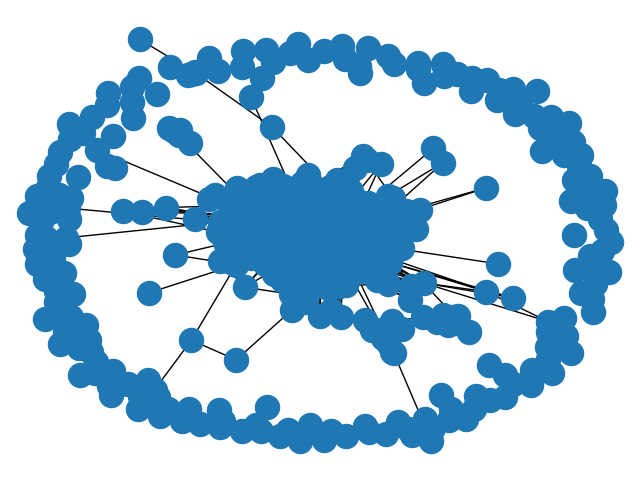
\includegraphics[scale=0.5]{G_weighted.png}
 	\label{fig:weighted_sim_graph}
 \end{figure}
 
 Next, we use the HCS algorithm to cluster data points in the graph. The result consists of five clusters that contain more than one data point, namely 2, 68, 140, 148 and 153. We reassign all samples located in singleton clusters to these five using the approach described in Subsection~\ref{subsec:singletons}. After this procedure, the clusters are populated as shown in Table~\ref{tab:pop_clusters_weighted} sorted by size in descending order. We can see that we have three larger groups and two smaller ones. 

 \begin{table}
 	\caption{Population of the clusters for the weighted approach with $\sigma=150$ and  $\epsilon=0.6$}
 	\centering
 	\begin{tabular}{|c|c|}
 		\hline
 		class & size \\
 		\hline
 		2 & 136 \\
 		148 & 121 \\
 		68 & 118 \\
 		140 & 27 \\
 		153 & 21 \\
 		\hline
 	\end{tabular}
 	\label{tab:pop_clusters_weighted}
 \end{table}
 
 To get a feeling if these clusters acutally make sense from a practical point of view, we take a look at how they are distributed among the true cancer types that we chose for this implementation, namely 'KIRC', 'LUAD' and 'PRAD'. In Figure~\ref{chart:distr_clustering_labels} we show the results. We observe that execpt for $1\%$ of the observations in class 'KIRC' the clustering achieved a strong seperation of the classes which is in agreement with the results of Section~\ref{sec:properties_HCS}. Additionally, we can see that within the classes 'KIRC' and 'LUAD' the clustering algorithm respectively seperated almost one fifth of the samples from the rest. This can lead us to the assumption that the algorithm is in fact capable of identifying cancer subtypes which, as we pointed out in Chapter~\ref{ch:intro}, is very useful for the development of more personalized cancer treatments.

\begin{figure}
	\caption{Distribution of the clustering labels among the cancer type classes for the weighted approach with $\sigma=150$ and  $\epsilon=0.6$}
	\centering
	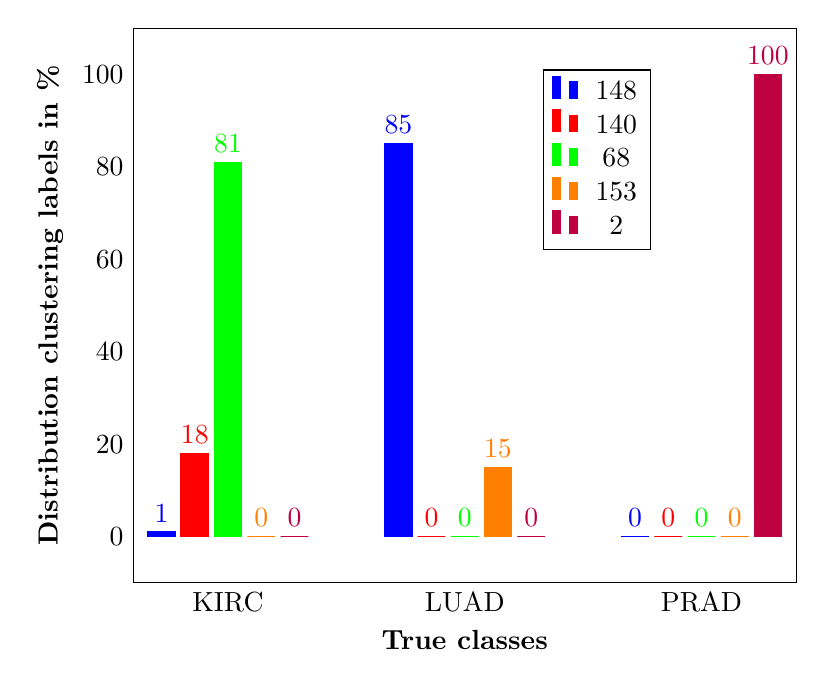
\begin{tikzpicture}
		\begin{axis}
		[
		ybar,
		xtick=data,
		tickwidth         = 0pt,
		enlarge x limits  = 0.2,
		nodes near coords,
		symbolic x coords = {KIRC,LUAD, PRAD},
		legend style = {at={(0.7, 0.6)}, anchor=south, column sep=1ex},
		ylabel=\textbf{Distribution clustering labels in \%},
		xlabel=\textbf{True classes},
		]
		\addplot[style={blue, fill=blue}] coordinates { (KIRC, 1) (LUAD, 85) (PRAD, 0)};
		\addplot[style={red, fill=red}] coordinates { (KIRC, 18) (LUAD, 0) (PRAD, 0)};
		\addplot[style={green, fill=green}] coordinates { (KIRC, 81) (LUAD, 0) (PRAD,0)};
		\addplot[style={orange, fill=orange}] coordinates { (KIRC, 0) (LUAD,15) (PRAD, 0)};
		\addplot[style={purple, fill=purple}] coordinates { (KIRC, 0) (LUAD, 0) (PRAD, 100) };
		\legend{148, 140, 68, 153, 2}
		\end{axis}
	\end{tikzpicture}
	\label{chart:distr_clustering_labels}
\end{figure}

\subsection{Non-weighted similarity graph}
As for the weighted approach, we constructed the similarity graph as shown in Figure~\ref{fig:unweighted_sim_graph}. In the picture of the graph in comparison to the one from the weighted approach, we can definitely see more edges but when looking at the data points forming the circle-like shape, we observe that it is in fact bigger than the one for the weighted approach. This means that the component displayed in the center of the non-weigthed graph is less populated and thus, we can see more edges when in fact this graph has actually less due to the choice of parameters.

\begin{figure}
	\centering
	\caption{Non-weighted $0.7$-neighborhood similarity graph with $\sigma=150$}
	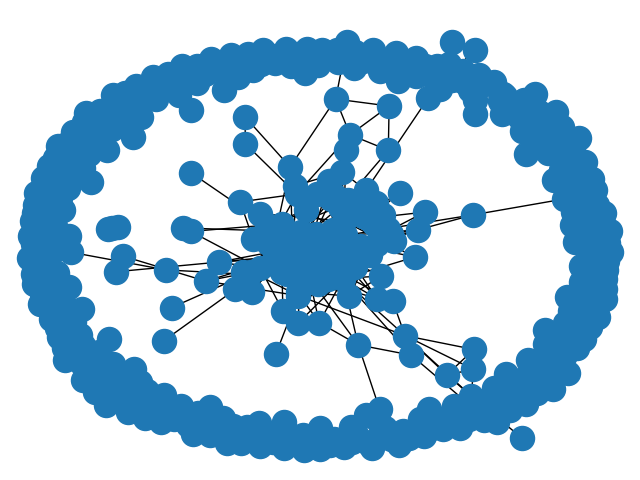
\includegraphics[scale=0.5]{G_unweighted.png}
	\label{fig:unweighted_sim_graph}
\end{figure}

After applying the HCS algorithm and reassigning samples in singleton clusters, we get four clusters, namely 10, 21, 31 and 72. Their populations are shown in Table~\ref{tab:pop_clusters_unweighted}.

\begin{table}
	\caption{Population of the clusters for the unweighted approach with $\sigma=150$ and  $\epsilon=0.7$}
	\centering
	\begin{tabular}{|c|c|}
		\hline
		class & size \\
		\hline
		31 & 251 \\
		10 & 98 \\
		21 & 48 \\
		72 & 26 \\
		\hline
	\end{tabular}
	\label{tab:pop_clusters_unweighted}
\end{table}

Comparing the clustering results to the true classes, we see that the separation between the classes is not really given since both 'LUAD' and 'PRAD' are dominated by cluster label 31. Looking at the cluster sizes this is not surprising since we chose the three classes to have about the same size, yet cluster 31 contains more than half of all samples. Class 'KIRC' on the other hand seems to be well separated from the other two and also split into two subtypes but which have different distributions among the samples compared to the weighted approach. 

\begin{figure}
	\caption{Distribution of the clustering labels among the cancer type classes for the unweighted approach with $\sigma=150$ and  $\epsilon=0.7$}
	\centering
	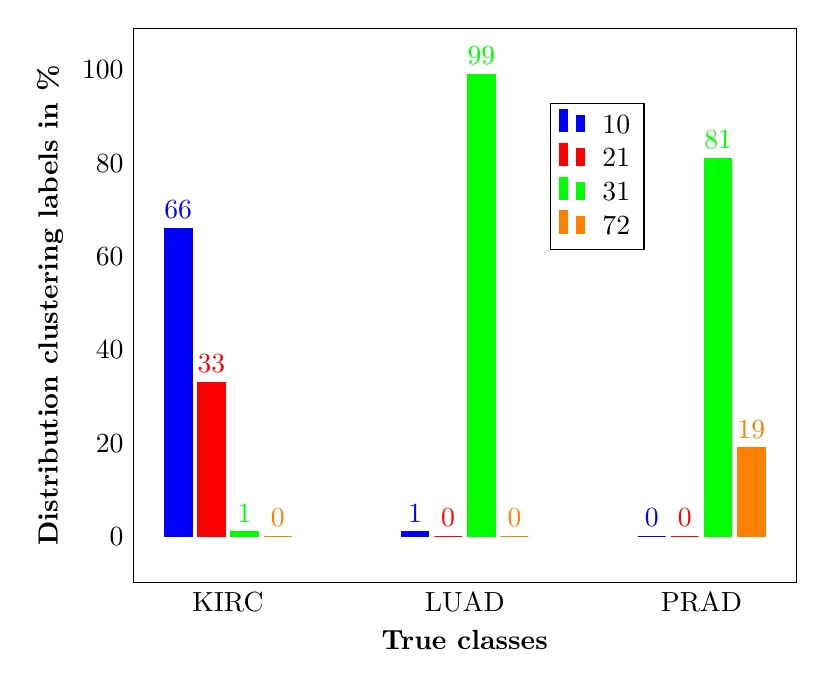
\begin{tikzpicture}
	\begin{axis}
	[
	ybar,
	xtick=data,
	tickwidth         = 0pt,
	enlarge x limits  = 0.2,
	nodes near coords,
	symbolic x coords = {KIRC,LUAD, PRAD},
	legend style = {at={(0.7, 0.6)}, anchor=south, column sep=1ex},
	ylabel=\textbf{Distribution clustering labels in \%},
	xlabel=\textbf{True classes},
	]
	\addplot[style={blue, fill=blue}] coordinates { (KIRC, 66) (LUAD, 1) (PRAD, 0)};
	\addplot[style={red, fill=red}] coordinates { (KIRC, 33) (LUAD, 0) (PRAD, 0)};
	\addplot[style={green, fill=green}] coordinates { (KIRC, 1) (LUAD, 99) (PRAD,81)};
	\addplot[style={orange, fill=orange}] coordinates { (KIRC, 0) (LUAD,0) (PRAD, 19)};
	\legend{10, 21, 31, 72}
	\end{axis}
	\end{tikzpicture}
	\label{chart:distr_clustering_labels_unweighted}
\end{figure}

Obviously, we have only looked at one example of parameters but still we notice the tendency that it yields better results to have more edges with weights than to reduce the computational time by taking the non-weighted approach with less edges.

\section{Choice of parameters}\label{sec:choice_para}
When we discussed the results of the algorithms applied to the RNA-Seq PANCAN data set, we chose a set for parameters mainly by intuition and even if the results were really good for the weighted approach the question still remains if there are other set of parameters that might lead to similarly good results but have different subclusters. In this case, other questions follow like how to choose based on some criterion the best solution or is it even desirable to have only one subclassification? One can imagine that the choice of which personalized treatment to apply to a certain patient might as well be the result of intersections of different subclassifications. 

These are questions that are most likely better answered by a biologist, but concretely in this situation we need to figure out a way to even get those other parameter settings with a comparable result. One approach could be to use hyperparamter optimization to obtain $\sigma$ and $\epsilon$. There are different approaches to consider, namely manual search, random search or grid search. Manual search seems to be a lot of work and since the algorithm runs a long time requires also a lot of waiting. Random search might be a bit like finding a needle in a hay stack since in our example we have seen that for $\sigma$ a wide range of values are reasonable choices. Additionally, we can give an indication in which interval $\epsilon$ should be given a $K$ matrix based on $\sigma$ because if all values are below some threshold it makes no sense to choose an $\epsilon$ that it above it. Thus, it is reasonable to apply the grid search hyperoptimization technique\footnote{In Python, this can be implemented using the 'scikit-learn' package's 'GridSearchCV()' function that is part of the 'model\_selection' function bundle. Further details and the documentation can be found at \url{https://scikit-learn.org/stable/modules/generated/sklearn.model_selection.GridSearchCV.html\#sklearn.model_selection.GridSearchCV}.} and also not to consider any automated hyperparameter tuning approaches at all since they are more helpful when one does not have additional knowledge about how to choose the hyperparameters. 

Naturally, after selecting the proper technique there are still a lot of choices left to make like the method of evaluating the different clustering results, of efficiently searching the parameter grid or of splitting in cross-validation. However, discussing these topics is beyond the scope of this project and at this point we just wanted to provide some outlook on potential improvements of the procedure described here.

\bibliographystyle{ieeetr}
\bibliography{literature_algo}
\end{document}